% -*- coding: utf-8 -*-
% !TEX program = xelatex
\documentclass{njustexam}

\usepackage{wrapfig}

%注意:注释掉这条命令则显示答案, 为存档用, 交教务处. 使用这条命令则为学生考试用, 交印刷厂印刷
% \answerfalse 

\begin{document}
%%%%%%%%%%%%%%%%% 以下内容根据需要更改%%%%%%%%%%%
\renewcommand{\course}{大学物理II}                          %课程名
\renewcommand{\duration}{120}                                            %考试时长
\renewcommand{\credit}{5}                                                   %学分
\renewcommand{\syllabus}{11220804-0}                               %教学大纲编号
\renewcommand{\fullmark}{100}                                            %满分分值
\renewcommand{\composer}{罗凯}            %组卷教师
\renewcommand{\composedate}{\today}                   %组卷日期
\renewcommand{\validator}{}                                        %审定人
\renewcommand{\coursetype}{1}                                            % 1 为必修, 0 为选修
\renewcommand{\exammethod}{1}                                         % 1 为闭卷, 0 为开卷
\renewcommand{\testpaper}{B}                                              % A 或 B
%%%%%%%%%%%%%%%%%%%%%%%%%%%%%%%%%%%%%%

\makehead % 生成试卷表头

\makepart{填空题}{共~8~小题, 每空~2~分, 共~40~分}

% 电磁学:

% 在真空中,光速的数值为 \underline{\hspace{2cm}} m/s。
% 静电场中,库仑力与电荷之间的关系由 \underline{\hspace{2cm}} 定律描述。
% 安培环路定理描述了 \underline{\hspace{2cm}} 和磁场之间的关系。
% 法拉第电磁感应定律描述了磁场变化引起的 \underline{\hspace{2cm}}。
% 电场的高斯定理表明,电场通过一个 \underline{\hspace{2cm}} 的闭合曲面的通量等于这个曲面内的电荷总量除以真空介电常数 $\varepsilon_0$。
% 光学:

% 光的波长与频率之间的关系由 \underline{\hspace{2cm}} 公式描述。
% 在光的折射现象中,折射率定义为光在介质中的速度与真空中的速度的 \underline{\hspace{2cm}}。
% 光的全反射现象发生在光线从折射率较大的介质射向 \underline{\hspace{2cm}} 折射率的介质时。
% 某个透镜的焦距是它的 \underline{\hspace{2cm}} 和介质折射率的函数。
% 杨氏双缝干涉实验中,光的干涉现象是由光的 \underline{\hspace{2cm}} 性质引起的。
% 现代物理:

% 量子力学中,波函数描述了粒子的 \underline{\hspace{2cm}}。
% 量子力学的基本方程是薛定谔方程,它描述了粒子的 \underline{\hspace{2cm}}。
% 物质波的频率与粒子的动量之间的关系由 \underline{\hspace{2cm}} 关系给出。
% 质能方程 $E=mc^2$ 揭示了质量与能量之间的 \underline{\hspace{2cm}}。
% 狭义相对论中,光速是一个 \underline{\hspace{2cm}} 常数。



\begin{problem} 
  本门课程《大学物理II》课堂每周\fillout{二}和周\fillout{四}的下午3:50--6:15。
\end{problem} 

% \begin{problem}
%   电流在空间产生磁场遵循的物理定律是\fillout{安培}定律。
% \end{problem} 

\begin{problem}
磁感应强度的单位是\fillout{特斯拉 (Tesla)或高斯 (Gauss)}。
\end{problem}


\begin{problem}
  安培环路定理描述了\fillout{电流}和\fillout{磁场}两个物理量之间的关系。
\end{problem}


\begin{problem}
  法拉第电磁感应定律定量描述了磁场变化引起\fillout{电势差或电动势}。
\end{problem}

\begin{problem}
薄膜干涉分为\fillout{等厚}干涉和\fillout{等倾}干涉;牛顿环属于\fillout{等厚}干涉,对应的图案为同心圆环。
\end{problem}

\begin{problem}
  常见光的衍射分为 \fillout{菲涅耳衍射}(即球面光波的衍射)和 \fillout{夫琅和费衍射}(即平面光波的衍射)。
 \end{problem}

 \begin{problem}
  现代物理的两个支柱理论是\fillout{量子力学}和\fillout{相对论}。
\end{problem}

% \begin{problem}
% 爱因斯坦因(Albert Einstein, 1879-1955)成功解释了\fillout{光电效应}获得1921年诺贝尔物理学奖。该解释采用了
% \fillout{普朗克}的量子假说。
% \end{problem}

% \begin{problem}
% 感应电动势分为\fillout{动生}电动势和\fillout{感生}电动势。 
% \end{problem}


  \begin{problem}

    关于顺磁介质的磁导率比真空的磁导率略\fillout{大}(填大或小)。
\end{problem}

\begin{problem}
  均匀磁场的磁感强度垂直于半径为r的圆面。今以该圆周为边线,作一半球面S(如图所示),则通过S面的磁通量的大小为: \fillout {$\pi r^2 B$}.
  % \begin{figure}[h]
    % \centering
    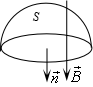
\includegraphics{Picture1.png}
  % \end{figure}
\end{problem}


% \begin{problem}
%   如图所示,电流从a点分两路通过对称的圆环形分路,汇合于b点,若ca、bd 都沿环的径向,则在环形分路的环心处的磁感应强度为 : \fillout {0}.
%   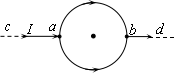
\includegraphics{Picture2.png}
% \end{problem}


% \begin{problem}
%   物质波是由\fillout{德布罗意}提出的,后来被实验验证,包括\fillout{电子衍射实验或汤姆逊}实验。
%   薛定谔方程的波函数$\Psi$的统计解释由\fillout{玻恩}给出,其模的平方$|\Psi|^2$表示\fillout{概率密度}。 
% \end{problem}


\begin{problem}
介质的折射率比空气折射率\fillout{大},介质中光速比真空中光速\fillout{小}
\end{problem}



% \begin{problem}

%   洛仑兹力不会:\pickout{A}
%   \begin{abcd}
%     \item 改变带电粒子的速率;  
%     \item 改变带电粒子的动量;
%     \item 改变带电粒子的速度;  
%     \item 改变带电粒子的加速度。
%   \end{abcd}
%   \end{problem}


  % \begin{problem}

  %     对于磁铁来说,磁畴(domain) 指的是:\pickout{C}
  %     \begin{abcd}
  %       \item 磁铁极间的区域
  %       \item 受磁场影响的磁铁周围空间
  %       \item 磁铁内部的区域,其中单个原子的磁极是对齐的
  %       \item 磁性材料开采的区域
  %     \end{abcd}
  % \end{problem}




% \begin{problem}

%   用细导线均匀密绕成的长为l,半径为a(l>>a),总匝数为N的螺线管通以稳恒电流I,当管内充满磁导率为的均匀磁介质后,管中任意一点:\pickout{D}
%   \begin{abcd}
%     \item 磁感应强度大小为 $B=\mu_0 \mu_r N I$

%     \item 磁感应强度大小为 $B=\mu_r N I / l $

%     \item 磁场强度大小为 $H=\mu_0 N I / l$

%     \item 磁场强度大小为 $H=N I / l$
%   \end{abcd}
% \end{problem}


% \begin{problem}
%   在稳恒磁场中, 有磁介质存在时的安培环路定理的积分形式是 : \pickout{B}
%   \begin{abcd}
%     \item  $\oint_L \vec{B} \cdot d \vec{l}=\sum_{\left(L_{\text {内 }}\right)} I$
%     \item  $\oint_L \vec{H} \cdot d \vec{l}=\sum_{\left(L_{\text {内 }}\right)} I$
%     \item  $\oint_L \vec{H} \cdot d \vec{l}=\mu_0 \sum_{\left(L_{\text {内 }}\right)} I$
%     \item  $\oint_L \vec{H} \cdot d \vec{l}=I_0+\iint_S \frac{\partial \vec{D}}{\partial t} \cdot d \vec{S}$
%   \end{abcd}

% \end{problem}


% \begin{problem}
%   半径为圆线圈置于磁感强度为的均匀磁场中,线圈平面与磁场方向垂直,线圈电阻为;当把线圈转动使其法向与夹角时,线圈中已通过电量与线圈面积及转动时间的关系是: 
% : \pickout{A}
%   \begin{abcd}
%     \item  与线圈面积成正比,与时间无关; 
%     \item  与线圈面积成正比,与时间成正比;
%     \item  与线圈面积成反比,与时间成正比;
%     \item  与线圈面积成反比,与时间无关;
%   \end{abcd}

% \end{problem}




% \begin{problem}

%     与霍耳效应(Hall Effect)的应用\textbf{不}符合的是:\pickout{A}
%     \begin{abcd}
%       \item 计算电子的电荷量
%       \item 判断半导体的类型
%       \item 测量磁场
%       \item 测量载流子浓度
%     \end{abcd}
% \end{problem}


% \begin{problem}

%   矢量叉乘(cross product)遵循的规则是:\pickout{B}
%   \begin{abcd}
%     \item 左手螺旋规则
%     \item 右手螺旋规则
%     \item 反常左手螺旋规则
%     \item 反常右手螺旋规则
%   \end{abcd}
% \end{problem}


\begin{problem}
杨氏双缝干涉实验中,光的干涉现象说明了光的\fillout{波动性}。
\end{problem}


\begin{problem}
一束波长为 $\lambda$ 的单色平行光垂直照射到宽的 $a$ 的单缝 $\mathrm{AB}$ 上, 
    若屏上的 $\mathrm{P}$ 为第三级明纹,则单缝 $A B$ 边缘 $A 、 B$ 两处光线之间的光程差为: \fillout{$7 \lambda / 2$}
\end{problem}
  
% \begin{problem}

%   量子力学中,波函数描述了粒子的:\pickout{D}
%   \begin{abcd}
%     \item 质量
%     \item 能量
%     \item 速度
%     \item 状态
%   \end{abcd}
% \end{problem}

% \begin{problem}

% 物质波的频率与粒子的动量之间的关系由哪个关系给出?\pickout{B}
% \begin{abcd}
%   \item 康普顿效应
%   \item 德布罗意关系
%   \item 波尔理论
%   \item 光电效应
% \end{abcd}
% \end{problem}

% \begin{problem}

%   质能方程 $E=mc^2$ 揭示了质量与能量之间的:\pickout{B}
%   \begin{abcd}
%     \item 相等关系
%     \item 变换关系
%     \item 成正比关系
%     \item 无关系
%   \end{abcd}
%   \end{problem}

\begin{problem}
能量为5.0eV的光子入射到某金属表面,测得光电子的最大初动能是1.5eV,为了使该金属能产生光电效应,则入射光子的最低能量为 \fillout{3.5}eV。                                              
    % \begin{abcd}
    %       \item  1.5eV 
    %       \item  2.5eV  
    %       \item  3.5eV   
    %       \item  5.0eV
    % \end{abcd}
\end{problem}

% \begin{problem}
% 杨氏双缝实验中,设想用完全相同但偏振化方向相互垂直的偏振片各盖一缝,则屏幕上干涉条纹强度为 \fillout{0}。 
% \end{problem}


% \begin{problem}
%   磁场方向与线圈平面垂直,且穿入纸面向内,设通过线
%   圈回路的磁通量依照$\Phi = 6t^2 + 7t + 1$; 式中,$\Phi$的单
% 位为毫韦伯 (mWb),$t$ 的单位为秒 (s),
% t=1s 时,在这回路
% 中的感应电动势大小为\fillout{$9\times 10^{-3}$} V; 此时的磁通量大小为\fillout{$14$} (mWb)。
% \end{problem}




\makepart{计算题}{共~60~分}%共~6~小题, 每小题~8~分, 共~48~分}

\begin{problem}{(10分)}
  某闭合三棱柱面如图所示,处于磁感应强度大小为、方向沿x轴正方向的均匀磁场中。
  已知ab = 40 cm, be = ad = 30cm,  ae = 50cm, 
   求:
  \begin{enumerate}[label=(\arabic*)]
    \item 通过图中 abcd 面的磁通量;
    \item 通过图中 befc 面的磁通量;
    \item 通过图中 aefd 面的磁通量;
  \end{enumerate}
  综上判断高斯定理是否满足。  
  \begin{flushright}
    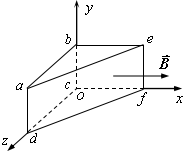
\includegraphics[width=0.15\textwidth]{Picture7.png}
  \end{flushright}
% \begin{wrapfigure}{r}{0.2\textwidth}
%   % \vspace{-20pt}
%   % \begin{center}
%     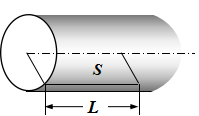
\includegraphics[width=0.1\textwidth]{Picture4.png}
%   % \end{center}
%   % \vspace{-20pt}
%   % \caption{A gull}
%   % \vspace{-10pt}
% \end{wrapfigure}

\end{problem}

\begin{solution}
\begin{enumerate}[label=(\arabic*)]
  \item $$\Phi_{a b c d}=B S_{a b c d} \cos \pi=-2 \times 0.30 \times 0.40=-0.24 (\mathrm{Wb}) \score{3}$$
  \item $$\Phi_{b e f c}=B \cdot S_{b e f c} \cdot \cos \frac{\pi}{2}=0  (\mathrm{Wb})\score{5}$$
  \item $$\Phi_{\text {aefd }}=B S_{a b c d}=0.24 (\mathrm{Wb}) \score{7}$$
\end{enumerate}
验证高斯定理: $$\oint_S \vec{B} \cdot d \vec{S}=\sum_{i=1}^5 \Phi_m^{(i)}=-0.24+0+0.24+0+0 (\mathrm{Wb}) =0 (\mathrm{Wb})$$
因此满足。\score{10}
\end{solution}


% \renewcommand{\solutionname}{证} % 将“解"字改为“证"字

% \begin{problem}{(6分)}
%   设 $\Psi(t,  x)=e^{ 2 t x-t^2 }$,  $t$是复变数,  证明: 
%   $$
%   \left. \frac{\partial^n \Psi(t,  x)}{\partial t^n}\right|_{t=0}=(-1)^n e^{x^2} \frac{d^n}{\dx^n} e^{-x^2}
%   $$
%   % 提示: 对回路积分进行积分变数的代换 $\xi=z-x$. 
% \end{problem}

\begin{problem}{(10分)}
  一螺绕环,横截面的半径为a,中心线的半径为R ,R $\gg$ a ,其上由表面绝缘的导线均匀地密绕两个线圈,一个$N_1$匝,另一个$N_2$匝。
  求(1) 两线圈的自感$L_1$和$L_2$; (2) 两线圈的互感M。(3) M与$L_1$和$L_2$的关系。
\end{problem}
\vfill

\begin{solution}
% \everymath{\displaystyle}%
\? (1) 假设 1 线圈通电流为 $I_1$. \\ 
\+ 则 $$B_1=\frac{\mu_0 N I_1}{2 \pi R} \score{2}$$  
\+ $$\Phi_{11}=B_1 \cdot \pi a^2=\mu_0 \frac{N_1}{2 \pi R} I_1 \cdot \pi a^2$$
\+ 根据自感的定义
$$ L_1=\frac{N_1 \Phi_{11}}{I_1}=\frac{\mu_0 N_1^2}{2 \pi R} \cdot \pi a^2=\frac{\mu_0 N_1^2 a^2}{2 R} \score{4} $$
同理可得,
$$ L_2=\frac{N_2 \Phi_{22}}{I_2}=\frac{\mu_0 N_2{ }^2}{2 \pi R} \cdot \pi a^2=\frac{\mu_0 N_2{ }^2 a^2}{2 R} \score{6} $$
\+ (2) 根据互感的定义$$
M=M_{21}=\frac{\Psi_{21}}{I_1}=\frac{N_2 \frac{\mu_0 N_1 I}{2 \pi R} \pi a^2}{I_1}
$$
\+  最终结果为
$$ M =\frac{\mu_0 N_1 N_2}{2 R} a^2\score{8}$$ 
\+ (3) 它们满足$$M^2 = L_1 L_2 \score{10} $$
\end{solution}


% \begin{problem}{(10分)}
%   电流I均匀地流过一根截面半径为R的长直铜导线。在导线内部取一平面S,一边为轴线,另一边在导线外壁上,长度为L,试求  
%   \begin{enumerate}
%     \item 磁感应强度分布
%     \item 通过面S的磁通量
%   \end{enumerate}
% % \begin{wrapfigure}{c}{0.2\textwidth}
% %   \vspace{-20pt}
% %   \begin{center}
% %     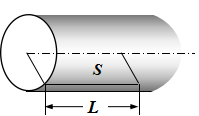
\includegraphics[width=0.2\textwidth]{Picture4.png}
% %   \end{center}
% %   \vspace{-20pt}
% %   \caption{A gull}
% %   \vspace{-10pt}
% % \end{wrapfigure}

%     \begin{flushright}
%       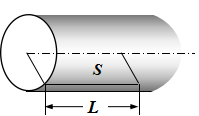
\includegraphics[width=0.2\textwidth]{Picture4.png}
%     \end{flushright}
% \end{problem}


% \begin{solution}
%   函数$\bar{f}(p)$可以写成
%   $$
%   \bar{f}(p) = \frac{3}{2} \left[ \frac{1}{p+1} + \frac{1}{p-1}  \right] \score{3}
%   $$
%   由拉普拉斯变换的定义不难得到$$\mathcal{L}^{-1} \left[ \frac{1}{p-s} \right] = e^{st}, $$
%   故得到
%   $$\mathcal{L}^{-1} \left[ \frac{1}{p+1}\right] = e^{-t} $$
%   和
%   $$\mathcal{L}^{-1} \left[ \frac{1}{p-1}\right] = e^{+t} \score{5}  $$
%   根据双曲余弦函数的定义, 最终我们有原函数
%   $$f(t) =\mathcal{L}^{-1} \left[ \bar{f}(p) \right] = 3\cosh t.  \score{7}$$
% \end{solution}
  
\begin{problem}{(10分)}
  如图所示, 一磁导率为 $\mu_1$ 的无限长磁介质圆柱体, 其半径为 $R_1$, 
  其中通有电流 $I$, 且电流沿横截面均匀分布。
  在该磁介质圆柱的外面有一半径为 $R_2$ 的无限长同轴圆柱面,二者之间充满磁导率为 $\mu_2$ 的均匀磁介质, 
  圆柱面外为真空。在圆柱面上通有相反方向的电流$I$。
  试求:
 \begin{enumerate}[label=(\arabic*)]
    \item  圆柱体内 $\left(r<R_1\right)$ 任一点的磁感应强度 $\boldsymbol{B}$;
    \item 圆柱体外与圆柱面内 $\left(R_1<r<R_2\right)$ 任一点的磁感应强度 $\boldsymbol{B}$;
    \item 圆柱面外 $\left(r>R_2\right)$ 任一点的磁感应强度 $\boldsymbol{B}$ 。
 \end{enumerate}
  \begin{flushright}
    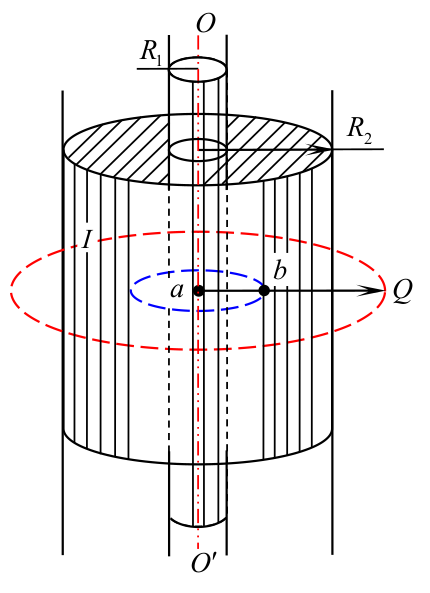
\includegraphics[width=0.15\textwidth]{Picture5.png}
  \end{flushright}
\end{problem}
  \vfill
  

\begin{solution}
  % \everymath{\displaystyle}%
  \begin{enumerate}[label=(\arabic*)]
    \item   \? 设圆柱体内任一点 a 到轴的垂直距离为 r( $r < R_1$ ),
    在垂直于圆柱轴的平面上,以轴与平面的交点为圆心,r 为半径作圆,取该圆周为积分回路,根据对称
    性可知,圆周上各点 H 的方向沿着圆的切线方向,与电流 I 满足右手螺旋;圆周上各点 H 的大小相等。
    应用有磁介质时的安培环路定理有 \score{1}
    $$
    \oint_L \boldsymbol{H}_1 \cdot d \boldsymbol{l}=H_1 \int_0^{2 \pi r} 
    d l=H_1 \cdot 2 \pi r=\sum I=\frac{I}{\pi R_1^2} \cdot \pi r^2=I \frac{r^2}{R_1^2} \score{4}
    $$
    \+由此得: 
    $$H_1=\frac{I r}{2 \pi R_1^2}$$; 
    \+ 由 $B=\mu_1 H_1$, 得: 
    $$B_1=\mu_1 H_1=\frac{\mu_1 I r}{2 \pi R_1^2}; \score{6}$$
    \item 同理, 当 $R_1<r<R_2$ 时, 根据有磁介质时的安培环路定理得
    $$\oint_L \boldsymbol{H}_2 \cdot d \boldsymbol{l}=H_2 \int_0^{2 \pi r} d l=H_2 \cdot 2 \pi r=\sum I=I $$
    $$\Rightarrow H_2=\frac{I}{2 \pi r}, $$
    $$ B_2=\mu_2 H_2=\frac{\mu_2 I}{2 \pi r} ; \score{8}$$
    \item 同理,当 $r > R_2$ 时,根据有磁介质时的安培环路定理得
    $$\oint_L \boldsymbol{H}_3 \cdot d \boldsymbol{l} = \sum I = 0$$
    $$\Rightarrow H_3=0 $$
    $$ B_3 = \mu_0 H_3 = 0 \score{10}$$.
  \end{enumerate}
\end{solution}

\begin{problem}{(10分)}
  用复色光源来做双缝实验,这种复色光由两种波长的光构成,$\lambda_1=$5500 Å。已知双缝间距为 0.60mm,
  屏和缝的距离为 1.20m,求屏上$\lambda_1$ 的第三级明纹极大位置。如屏上$\lambda_1$的第六级明纹极大和未知波长$\lambda_2$
  的第五级明纹极大重合,求未知光的波长$\lambda_2$。
\end{problem}

\begin{solution}
  \? 明纹的位置为 $$\quad x_k= \pm k \frac{D \lambda}{2 a}, \quad(k=0,1,2, \cdots) \score{3}$$
  \+(1) 第三级明纹极大位置为 
  $$ x_3=\frac{3 D \lambda_1}{2 a}=\frac{3 \times 1.2 \times 5500 \times 10^{-10}}{0.6 \times 10^{-3}}=3.3(\mathrm{~mm}) \score{6}$$
  \+ (2) 未知光的波长为 $\lambda_2$, 由题意有 $$\frac{6 D \lambda_1}{2 a}=\frac{5 D \lambda_2}{2 a} \score{8}$$
   $$\lambda_2=\frac{6 \lambda_1}{5}=6600(\text{\AA}) \score{10}$$
\end{solution}
\vfill


% \begin{problem}{(20分)}
%   一导线矩形框的平面与磁感强度为 $\boldsymbol{B}$ 的均匀磁场相垂直。
%   在矩形框上,有一质量 m,长为 l,可移动的细导体棒 MN,
%   矩形框还接有一个电阻 R,其值较之导线的电阻值要大得很
%   多。若开始时,细导体棒以速度 $v_0$沿如图所示的矩形框运动。
%   试求:
%   \begin{enumerate}[label=(\arabic*)]
%     \item 棒中的感应电动势
%     \item 棒所受的安培力
%     \item 棒的速率随时间变化的函数关系;
%     \item 棒移动的距离 随时间变化的函数关系;
%     \item 棒能移动的最大距离;
%     \item 从棒开始运动到任意 t 时刻回路中所产生的焦耳热。
%   \end{enumerate}
%   \begin{flushright}
%     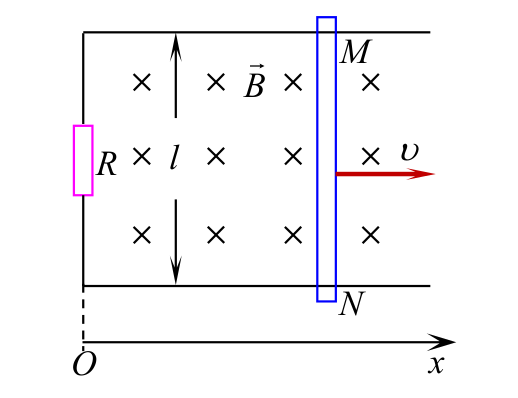
\includegraphics[width=0.2\textwidth]{Picture6.png}
%   \end{flushright}
% \end{problem}


% \begin{solution}
%   \begin{enumerate}[label=(\arabic*)]
%     \item 导体棒运动时产生感生电动势 $$\varepsilon=l B \frac{d x}{d t}=v B l \score{3} $$
%     \item 回路中的电流 
%     $$\quad i=\frac{\varepsilon}{R}=\frac{v B l}{R}$$ 
%     导体棒所受的安培力 
%     $$f=i B l=\frac{v B^2 l^2}{R} \score{6}$$
%     \item $$f=m a, \quad-\frac{v B^2 l^2}{R}=m \frac{d v}{d t}$$, 
%     解之得 $$v=v_0 e^{\frac{-B^2 l^2 t}{m R}} \score{9}$$
%     \item $v=v_0 e^{\frac{-B^2 l^2 t}{m R}}=\frac{d x}{d t}$, 
%     解之得 
%     $$x=\left(-\frac{v_0 m R}{B^2 l^2} e^{\frac{-B^2 l^2 t}{m R}}\right)_0^t
%     =\frac{v_0 m R}{B^2 l^2}\left(1-e^{\frac{-B^2 l^2 t}{m R}}\right) \score{12}$$
%     \item 当 $v=0$ 时, 即 $t \rightarrow \infty$ 时导体棒停下来, 则 
%     $$x_{\text {max }}=\lim _{t \rightarrow \infty} x=\frac{v_0 m R}{B^2 l^2} \score{15}$$
%     \item $$d W=i^2 R d t=\frac{l^2 B^2 v^2}{R^2} R d t=\frac{l^2 B^2}{R}\left(v_0 e^{\frac{-B^2 l^2 t}{m R}}\right)^2 d t \score{17} $$
%     $$
%     W=\int_0^t \frac{l^2 B^2}{R}\left(v_0 e^{\frac{-B^2 l^2 t}{m R}}\right)^2 d t 
%     =\left.\frac{l^2 B^2}{R} v_0^2\left(-\frac{m R}{2 l^2 B^2}\right) e^{\frac{-2 B^2 l^2 t}{m R}}\right|_0 ^t
%     =\frac{1}{2} m v_0^2\left(1-e^{\frac{-2 B^2 l^2 t}{m R}}\right) \score{20}
%     $$
%   \end{enumerate}
% \end{solution}





\begin{problem}{(20分)}
  宽度为 $a=0.6 \mathrm{~mm}$ 的狭缝后放置一焦距为 $f=40 \mathrm{~cm}$ 的凸透镜, 若以单色平行光垂直入射, 则在距中央明纹中心 $1.6 \mathrm{~mm}$ 处观察到红色明条纹,
   求(1)单色光波长; (2) 中央明纹宽度; (3) 第二级明纹对应的衍射角。
 \end{problem}

\begin{solution}
  (1) \? 单缝衍射明纹条件 $$a \sin \varphi_k= \pm(2 k+1) \frac{\lambda}{2}, \quad(k=1,2, \cdots) \score{3} $$ 
  
  第 $k$ 级明纹位置 $$
  x_k=f \cdot \tan \varphi_k \approx f \cdot \sin \varphi_k=\frac{2 k+1}{2} \cdot \frac{\lambda f}{a}, $$
  $$ \lambda=\frac{2 a x_k}{(2 k+1) f} \score{6} $$
$$
\begin{aligned}
& k=1, \lambda_1=\frac{2 a x}{3 f}=1600 \mathrm{~nm} \text { (不可见), } k=2, \lambda_2=\frac{2 a x}{5 f}=960 \mathrm{~nm} \text { (不可见), } \\
& k=3, \lambda_3=\frac{2 a x}{7 f}=686 \mathrm{~nm} \text { (红色), } k=4, \lambda_4=\frac{2 a x}{9 f}=533 \mathrm{~nm} \text { (绿色), }
\end{aligned}\score{10}
$$

所以在 $1.6 \mathrm{~mm}$ 处出现的是红光的第 3 级明纹。\score{12}

(2) \+ 由单缝衍射暗纹条件 $$a \sin \varphi_{1 \text {,暗 }}=\lambda , $$
 得 $$\sin \varphi_{1 \text {,暗 }}=\frac{\lambda}{a}, \score{14}$$
$$
l_0=2 x_{1 \text {,暗 }}=2 f \cdot \tan \varphi_{1 \text {, 暗 }}=\frac{2 \lambda f}{a}=\frac{2 \times 686 \times 10^{-9} \times 40 \times 10^{-2}}{0.6 \times 10^{-3}}=0.91(\mathrm{~mm})
\score{16}
$$
(3) \+ 单缝衍射明纹条件中, 取 $k=2$, 得 $$a \sin \varphi_2=\frac{5 \lambda}{2}, \score{18}$$
$$
\varphi_2 \approx \sin \varphi_2=\frac{5 \lambda}{2 a}=\frac{5 \times 686 \times 10^{-9}}{2 \times 0.6 \times 10^{-3}}=2.86 \times 10^{-3}(\mathrm{rad})=0.164^{\circ} \score{20}
$$
\end{solution}

% \begin{problem}{(10分)}
%   宽度为 $a=0.6 \mathrm{~mm}$ 的狭缝后放置一焦距为 $f=40 \mathrm{~cm}$ 的凸透镜, 若以单色平行光垂直入射, 
%   则在距中央明纹中心 $1.6 \mathrm{~mm}$ 处观察到红色明条纹,
%    求(1)单色光波长;(2)中央明纹宽度; (3) 第二级明纹对应的衍射角。
% \end{problem}
%   \vfill


% \begin{solution}
% 由边界条件可知该问题为轴对称情况
% 通解形式为
% $$  u(r,  \theta) = \sum_{l=0}^{\infty} \left( A_l r^l + \frac{B_l}{r^{l+1}} \right) P_{l} (\cos \theta). 
% $$
% 由$r=0$处有限的边界条件可知$B_l=0$.  \score{2}\\
% 因此, 对$r=a$处的边界条件带入, 得
% $$
% \sum_{l=0}^{\infty}  A_l r^l  P_{l} (\cos \theta) 
% = u_0 \cos^2 \theta = u_0 x^2 \score{4} 
% $$ 
% 勒让德多项式中$$P_0(x) = 1,  P_1(x) = x,  P_2 (x) = \frac{1}{2}(3x^2 - 1)$$ \\
% 不难得到 $$x^2 = \frac{2}{3} P_2(x) + \frac{1}{3} P_0(x), \score{6}$$  \\
% 比较两边系数, 得
% $$A_0 = \frac{u_0}{3}, \\
%  A_2 = \frac{2 u_0}{3a^2}, \\
%   A_l = 0 (l\neq 0,  2).  \score{8} $$ 
% 这样, 
% $$u(r, \theta) = \frac{u_0}{3} + \frac{2 u_0}{3a^2} r^2 P_2(\cos \theta).  \score{10} $$ 
% \end{solution}

\vfill
\newpage
\makedata{常用物理常数} %附录数据
\begin{itemize}
% 咐常用物理常数
\item 电子静止质量 $m_0=9.1 \times 10^{-31}(\mathrm{Kg})$ 
\item 电子电量 $e=1.6 \times 10^{-19}(C) \quad 1 \mathrm{eV}=1.60 \times 10^{-19} \mathrm{~J}$
\item 普朗克常数 $h=6.626 \times 10^{-34}(\mathrm{~J} \cdot \mathrm{s}) \quad$ 
\item 真空中光速 $c=3 \times 10^8(\mathrm{~m} / \mathrm{s})$
\item 维恩位移常数 $b=2.897 \times 10^{-3}(\mathrm{~m} \cdot \mathrm{K}) \quad$ 
\item 斯特藩常数 $\sigma=5.67 \times 10^{-8}\left(\mathrm{~W} \cdot \mathrm{m}^{-2} \cdot \mathrm{K}^{-4}\right)$
\item 真空磁导率 $\mu_0=4 \pi \times 10^{-7} \mathrm{~T} \cdot \mathrm{m} / \mathrm{A}$ 
\item 里德堡恒量 $R=1.096776 \times 10^7 \mathrm{~m}^{-1}$
\end{itemize}
% \begin{itemize}
%   \item 斯忒藩一坡耳兹曼定律: $E_B(T)=\sigma T^4, \quad \sigma=5.67 \times 10^{-8} \mathrm{~W} / \mathrm{m}^2 \cdot K^4$

%   \item  唯恩位移定律: $\lambda_m \cdot T=b, b=2.897 \times 10^{-3} m \cdot K$ 粒子的能量: $E=m c^2=h v$
%   \item  粒子的动量: $P=m v=\frac{h}{\lambda}$
%   \item 爱因斯坦方程: $h v=\frac{1}{2} m v^2+A$
%   \item 光子: $\varepsilon=h v, P=\frac{h}{\lambda}$
%   \item  两个公式: $r_n=\frac{\varepsilon_0 h^2 n^2}{\pi m e^2}=0.529 n^2 \stackrel{o}{A}$
%   \item 测不准关系 $\quad \Delta x \cdot \Delta P_x \geq h$
%   \item 红限频率: $v_0=\frac{A}{h}$
%   \item 玻尔假设: 定态, $L=n \cdot \frac{h}{2 \pi}=n h, h v=\left|E_n-E_m\right|$
%   \item $E_n=-\frac{m e^4}{8 \varepsilon_0{ }^2 h^2} \cdot \frac{1}{n^2}=\frac{-13.6}{n^2} e V \quad n=1,2,3, \cdots \cdots$
% \end{itemize}
\end{document}
